\documentclass[10pt,a4paper]{article}
\usepackage[spanish,es-nodecimaldot]{babel}
\usepackage[utf8]{inputenc}
\usepackage[T1]{fontenc}
\usepackage{lmodern}
\usepackage[margin=2cm]{geometry}
\usepackage{amsmath,amssymb}
\usepackage{graphicx}
\usepackage{booktabs,tabularx,array}
\usepackage{caption}
\usepackage{enumitem}
\usepackage{microtype}
\usepackage{placeins}
\usepackage{fancyhdr}
\usepackage{hyperref}

\hypersetup{
  colorlinks=true,
  linkcolor=black,
  urlcolor=blue!55!black,
  pdftitle={samIRA - Analítica y pronóstico de IRA en Puno}
}
\setlength{\parindent}{0pt}
\setlength{\parskip}{4pt}
\setlength{\headheight}{14pt}
\setlength{\emergencystretch}{3em}
\renewcommand{\arraystretch}{1.12}
\setlist{nosep,leftmargin=*}
\captionsetup{font=small,labelfont=bf,skip=4pt}
\pagestyle{fancy}
\fancyhf{}
\fancyhead[L]{\footnotesize samIRA -- Analítica de IRA}
\fancyhead[R]{\footnotesize Puno, Perú}
\fancyfoot[C]{\thepage}

\begin{document}

% Identificación académica
\begin{center}
{\Large\bfseries Inteligencia de negocios y aprendizaje automático para el análisis y pronóstico de infecciones respiratorias agudas en menores de cinco años en Puno, Perú (2000--2025)\par}
\vspace{0.2cm}
{\normalsize Proyecto samIRA}\par
\vspace{0.15cm}
\small
\textbf{Estudiante:} Maquera Andrade Aldair Jose \quad
\textbf{Docente:} Dr. Torres Cruz Fred\\
\textbf{Curso:} Business Intelligence \quad
\textbf{Actividad:} Analítica + Modelos + Optimización\\
\textbf{Fecha:} Noviembre de 2026
\end{center}
\vspace{0.1cm}\hrule

% Introducción
\section{Introducción}

Las infecciones respiratorias agudas (IRA) constituyen un motivo relevante de notificación sanitaria infantil en Puno. Sus registros semanales presentan estacionalidad, diferencias entre provincias y cambios significativos entre períodos históricos. Analizar estas variaciones permite describir el comportamiento de la vigilancia epidemiológica y evaluar cuánto pueden anticiparse los episodios notificados. Sin embargo, el número de episodios registrados no representa necesariamente personas únicas, incidencia poblacional ni capacidad asistencial utilizada.

El proyecto \textbf{samIRA} analiza las notificaciones de IRA sin neumonía en menores de cinco años durante 2000--2025. Su objetivo es integrar las cuatro dimensiones de la analítica de negocios descriptiva, diagnóstica, predictiva y prescriptiva mediante un panel provincial depurado, modelos a una y cuatro semanas, experimentos de optimización, evaluación temporal y estimación de incertidumbre. La simulación final plantea escenarios ilustrativos de planificación, no recomendaciones clínicas ni decisiones automáticas de asignación de recursos.

% Datos y metodología
\section{Datos y metodología}

\subsection{Fuente, limpieza y estructura}

La fuente principal fue el conjunto oficial \textit{Vigilancia epidemiológica de Infecciones Respiratorias Agudas (IRA)}, publicado por el CDC Perú/MINSA en la Plataforma Nacional de Datos Abiertos. El archivo de trabajo, filtrado a las 13 provincias de Puno, contiene \textbf{126\,118 registros} y \textbf{2\,297\,378 episodios de IRA sin neumonía} en menores de cinco años. La unidad de análisis es una provincia durante una semana epidemiológica, no un paciente individual.

La depuración corrigió \textbf{3\,751 registros} con nombres distritales dañados: Muñani (1\,305; UBIGEO 210208), Nuñoa (1\,237; 210806) y Mañazo (1\,209; 210109). El calendario se conservó según las variables de año y semana proporcionadas por la fuente, sin reconstruirlo mediante un calendario ISO. Para 2000--2025 se identificaron 1\,357 semanas, incluidas semanas 53 en 2003, 2008, 2014, 2020 y 2025. El panel balanceado contiene $13\times1\,357=\mathbf{17\,641}$ combinaciones provincia--semana.

Se identificaron \textbf{153 combinaciones sin notificación} (0,87\% del panel). Se preservaron como \texttt{NaN}, pues una semana sin reporte no equivale a cero episodios. Para obtener características rezagadas se utilizó la última observación disponible anterior al origen de predicción (LOCF causal); las filas sin observación real de la variable objetivo no se incorporaron a las métricas, según el indicador \texttt{es\_evaluable}. Las ausencias se concentraron principalmente en los primeros años; Moho registró 39, San Antonio de Putina 21, Yunguyo 20 y El Collao 19.

\subsection{Diseño predictivo y evaluación}

Las particiones se establecieron según el año de la variable objetivo: \textbf{entrenamiento 2001--2022} ($N=14\,785$), \textbf{validación 2023--2024} ($N=1\,347$) y \textbf{prueba retrospectiva 2025} ($N=689$). El año 2000 suministró antecedentes para construir retardos. En entrenamiento, las 14\,924 filas teóricas menos 139 ausencias explican las 14\,785 observaciones evaluables. El horizonte $h=1$ predice la semana inmediata; $h=4$ predice directamente la cuarta semana futura, sin acumular cuatro semanas de episodios. En ambos casos las características se calculan con información disponible al origen del pronóstico ($t-h$ para una semana objetivo $t$).

Se compararon líneas base \textit{Naive}, \textit{Seasonal Naive} y ETS/Holt--Winters con LightGBM local, LightGBM global y XGBoost global. Estos últimos utilizaron retardos autorregresivos, medias y desviaciones móviles, estacionalidad anual, armónicas de Fourier, indicador del período 2020--2022 e identificación provincial. Las ejecuciones de los modelos de árboles y de Optuna utilizaron semilla 42. La selección de configuraciones se realizó en 2023--2024; 2025 no se empleó para ese ajuste original.

El desempeño puntual se midió mediante MAE, RMSE, WAPE y sesgo medio:
\begin{align}
\mathrm{MAE} &= \frac{1}{N}\sum_i|y_i-\hat y_i|, &
\mathrm{RMSE} &= \sqrt{\frac{1}{N}\sum_i(y_i-\hat y_i)^2},\\
\mathrm{WAPE}(\%) &=100\frac{\sum_i|y_i-\hat y_i|}{\sum_i y_i}, &
\mathrm{Bias} &=\frac{1}{N}\sum_i(\hat y_i-y_i).
\end{align}
Para los intervalos predictivos al 95\% se analizaron cobertura, amplitud y Winkler Score. Este último suma el ancho del intervalo y una penalización de $2/\alpha=40$ veces la distancia fuera de los límites, con $\alpha=0,05$. Un intervalo no es preferible únicamente por cubrir más observaciones: también importa su amplitud.

% Resultados
\section{Resultados y analítica}

\subsection{Analítica descriptiva: evolución y territorio}

La evolución departamental presenta tres períodos: 2000--2019, con una media de \textbf{1\,889,6 episodios semanales}; 2020--2022, con \textbf{728,7}; y 2023--2025, con \textbf{1\,350,9}. La reducción media entre los dos primeros períodos fue del \textbf{61,4\%}, seguida de una recuperación parcial. La Figura~\ref{fig:evolucion} permite ubicar esta ruptura dentro de la serie completa, sin atribuirla a una causa única.

\begin{figure}[htbp]
\centering
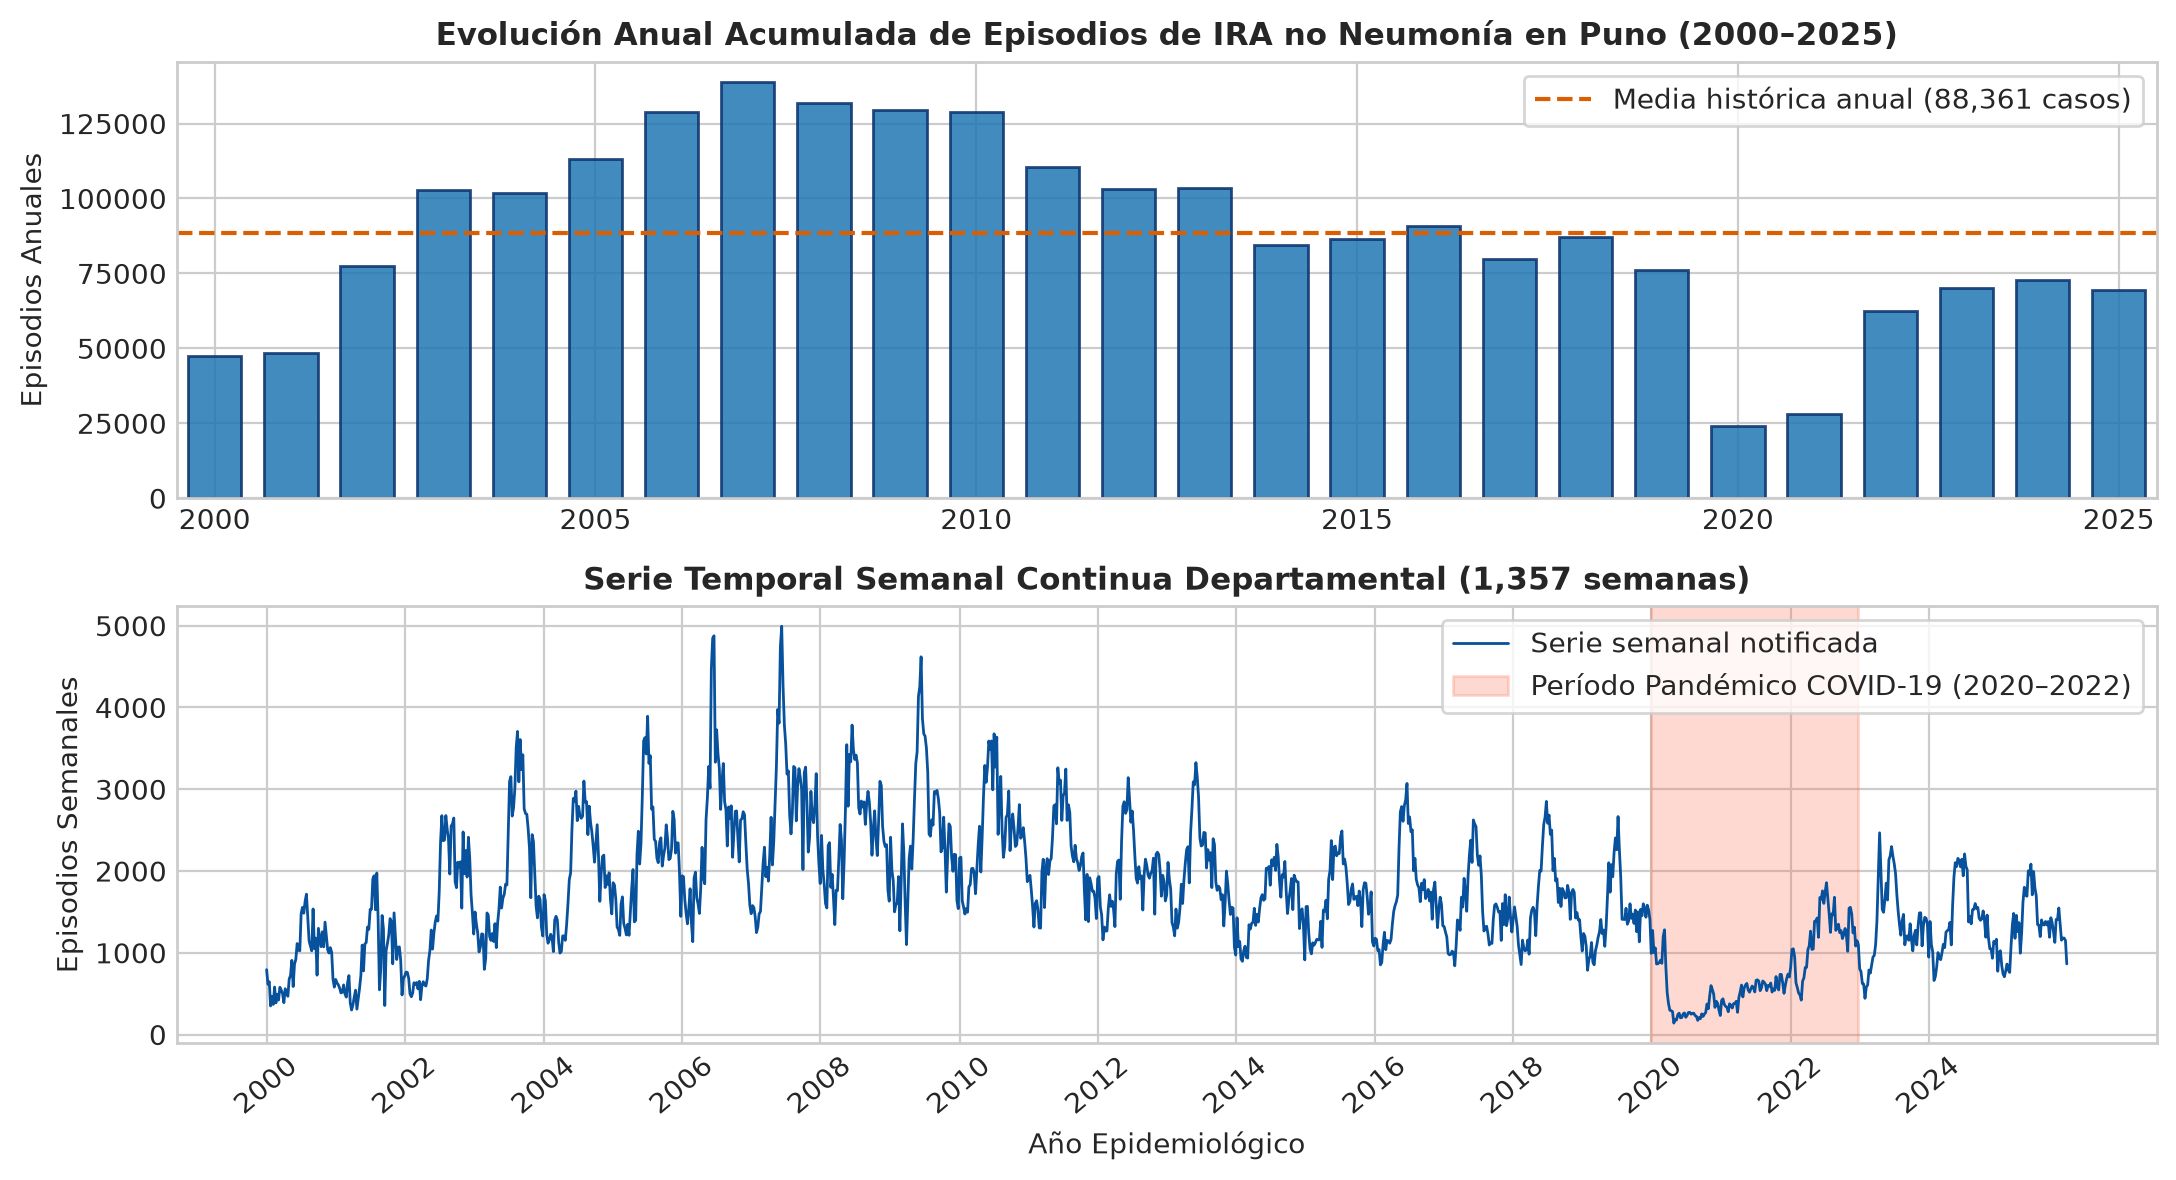
\includegraphics[width=0.95\linewidth,height=0.29\textheight,keepaspectratio]{figuras/01_evolucion_historica_ira.png}
\caption{Evolución histórica de los episodios notificados de IRA sin neumonía en Puno, 2000--2025.}
\label{fig:evolucion}
\end{figure}

La concentración territorial es marcada: \textbf{San Román} acumuló 569\,203 episodios (24,78\%), \textbf{Puno} 383\,892 (16,71\%) y \textbf{Azángaro} 254\,292 (11,07\%). Las dos primeras provincias reunieron el \textbf{41,49\%} del total; Moho, en contraste, registró 24\,018 (1,05\%). La Figura~\ref{fig:distribucion} compara la distribución absoluta. Sin denominadores poblacionales provinciales por edad, estas diferencias no pueden interpretarse como diferencias de riesgo individual.

\begin{figure}[htbp]
\centering
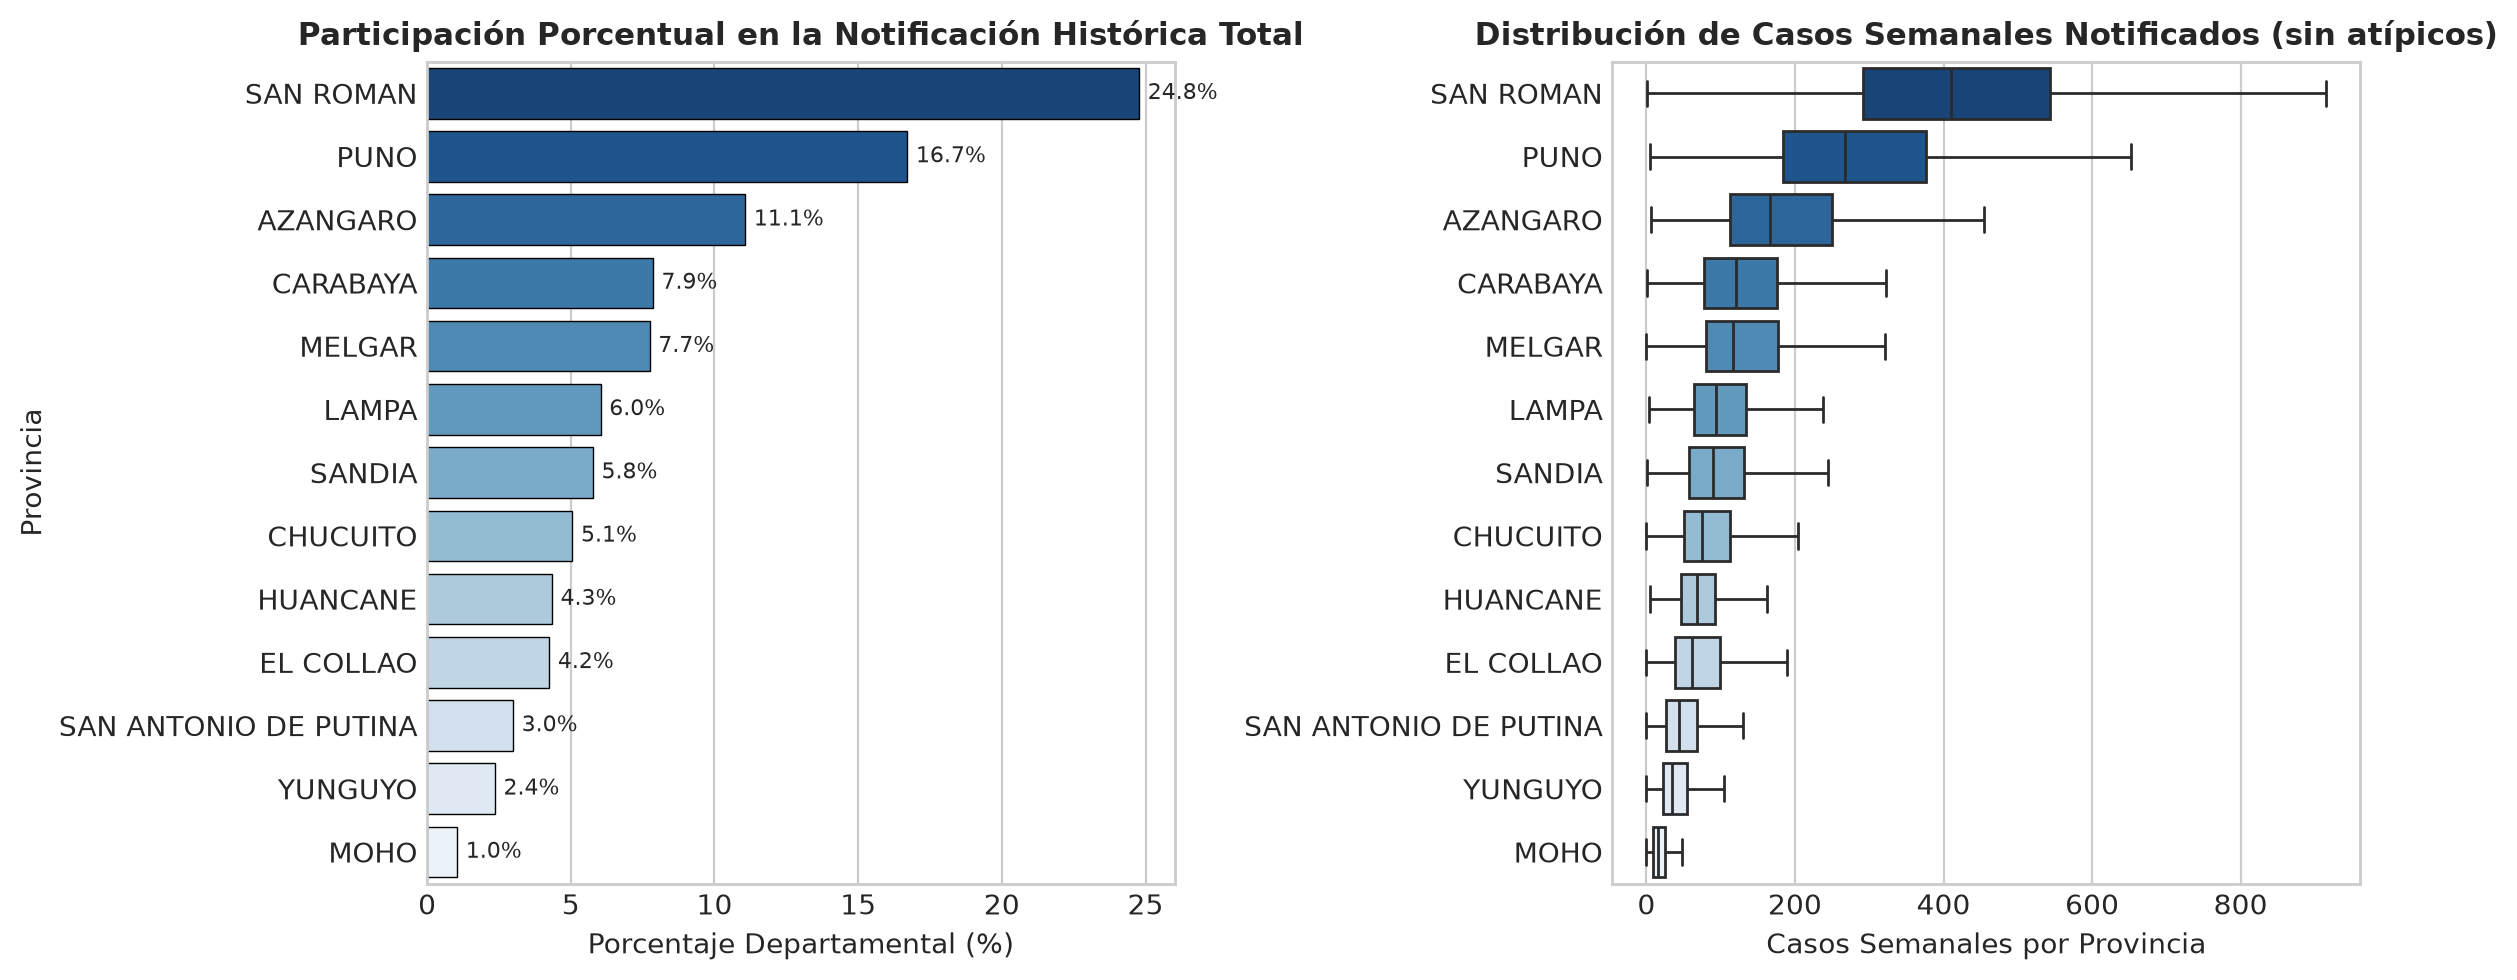
\includegraphics[width=0.95\linewidth,height=0.28\textheight,keepaspectratio]{figuras/02_distribucion_provincial_ira.png}
\caption{Concentración de episodios notificados y variabilidad semanal por provincia.}
\label{fig:distribucion}
\end{figure}

En el calendario semanal destaca una ventana de mayor actividad entre las \textbf{semanas 20 y 32}, con un máximo histórico promedio alrededor de la semana 26, de \textbf{2\,429,4 episodios regionales}. La dispersión interanual también aumenta en la temporada de mayor notificación (Figura~\ref{fig:estacionalidad}).

\begin{figure}[htbp]
\centering
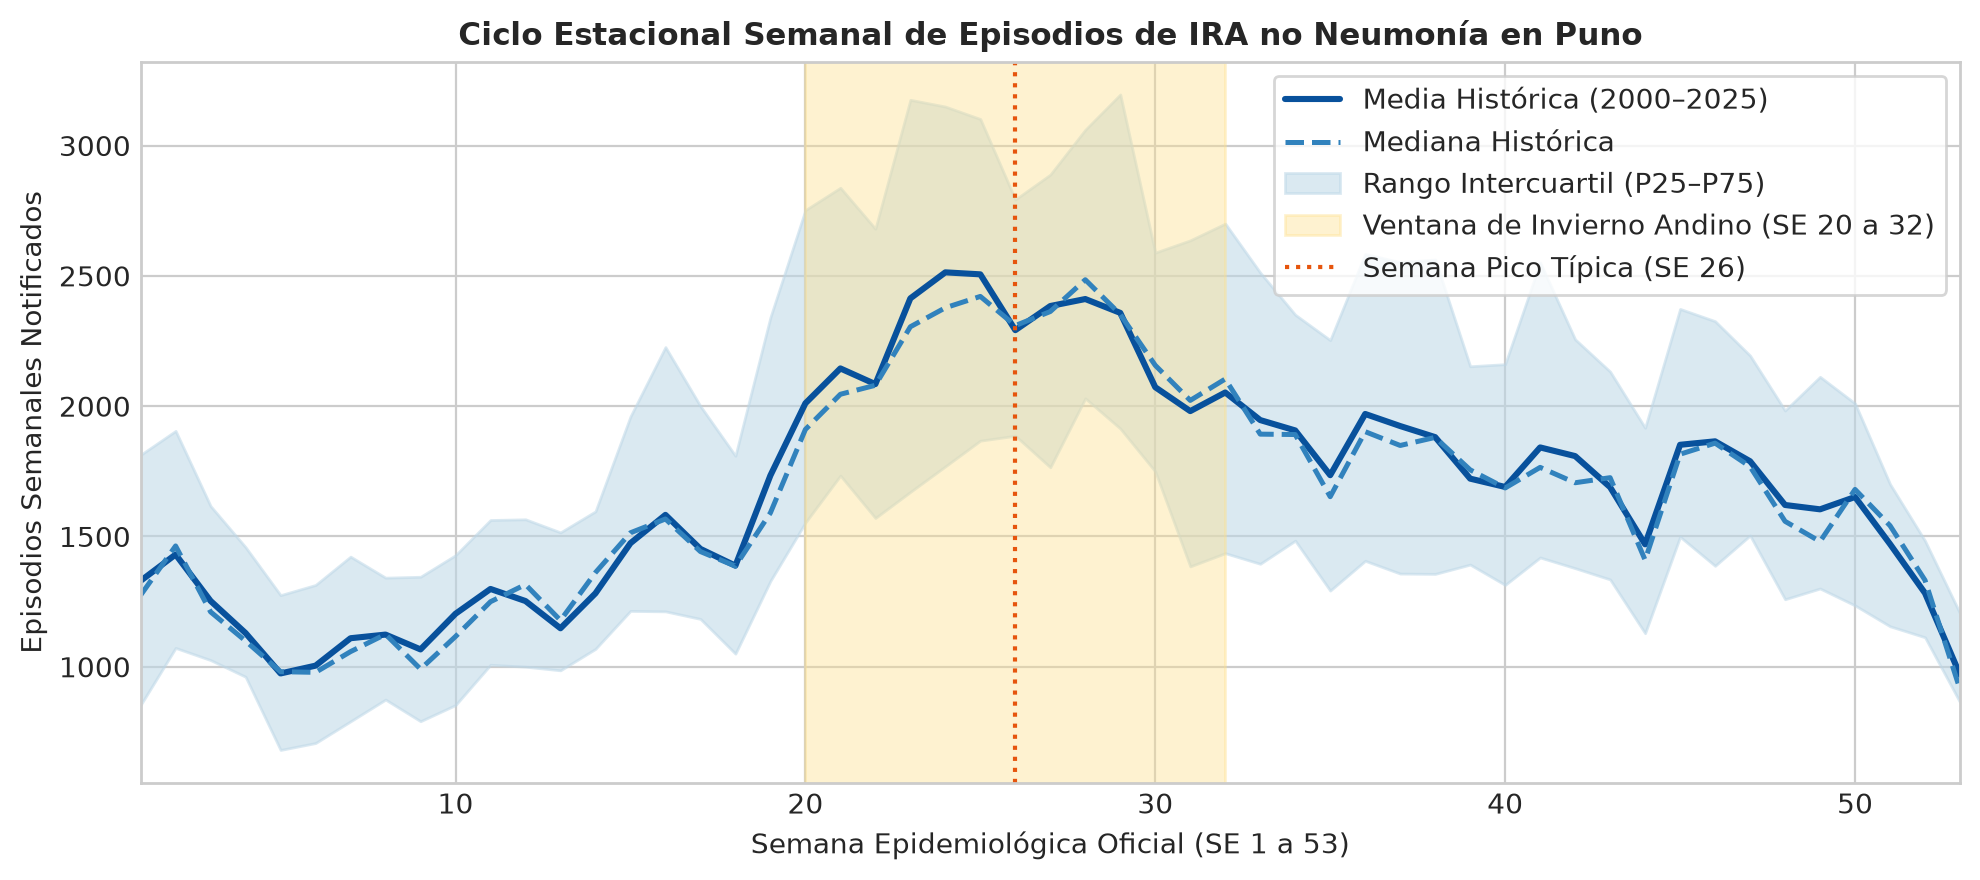
\includegraphics[width=0.95\linewidth,height=0.28\textheight,keepaspectratio]{figuras/03_estacionalidad_semanal.png}
\caption{Comportamiento estacional histórico según semana epidemiológica.}
\label{fig:estacionalidad}
\end{figure}

\subsection{Analítica diagnóstica: cambios y dispersión}

La reducción de 2020--2022 coincide temporalmente con la emergencia por COVID-19, pero los registros disponibles no distinguen cuánto corresponde a transmisión, acceso a servicios o cambios de notificación. Tampoco basta la coincidencia entre mayor notificación y meses fríos para estimar el efecto causal de la temperatura, pues el panel modelado no incorpora observaciones meteorológicas.

La relación marginal varianza/media del panel fue de \textbf{143,65}, con diferencias notables entre provincias; por ejemplo, Moho presentó un cociente de 8,24 y San Román de 87,38. Este estadístico agregado combina diferencias territoriales y temporales. La elevada dispersión y la desigualdad en los volúmenes anticipan una limitación analítica: una métrica regional favorable puede ocultar errores provinciales relevantes, y las tasas calculadas sobre pocos episodios requieren interpretación cautelosa.

\subsection{Analítica predictiva: comparación de modelos}

En validación 2023--2024, \textbf{LightGBM global} registró el menor WAPE en ambos horizontes: \textbf{18,247\%} ($h=1$) y \textbf{23,135\%} ($h=4$). En la prueba retrospectiva 2025, los menores errores observados correspondieron a \textbf{XGBoost global}: \textbf{15,718\%} y \textbf{18,972\%}, respectivamente. La Tabla~\ref{tab:modelos} conserva las métricas complementarias; la Figura~\ref{fig:modelos} resume la comparación de WAPE. Diferencias pequeñas entre algoritmos no prueban superioridad estadística sin un contraste adicional.

\begin{table}[htbp]
\centering
\caption{Modelos comparados en validación y prueba: MAE, RMSE y Bias en episodios; WAPE en porcentaje.}
\label{tab:modelos}
\footnotesize
\setlength{\tabcolsep}{4pt}
\begin{tabular}{llrrrr}
\toprule
\textbf{Período / $h$} & \textbf{Modelo} & \textbf{MAE} & \textbf{RMSE} & \textbf{WAPE} & \textbf{Bias}\\
\midrule
Val. 2023--24 / 1 & LightGBM global & 19,33 & 30,32 & \textbf{18,247} & +1,69\\
 & XGBoost global & 19,66 & 31,82 & 18,563 & +1,10\\
 & LightGBM local & 21,14 & 32,93 & 19,958 & +2,97\\
 & ETS & 21,18 & 33,73 & 19,996 & +0,21\\
 & Naive & 23,06 & 36,05 & 21,765 & $-0,05$\\
 & Seasonal Naive & 31,47 & 49,25 & 29,713 & $-7,44$\\
\midrule
Val. 2023--24 / 4 & LightGBM global directo & 24,51 & 39,32 & \textbf{23,135} & +4,98\\
 & XGBoost global directo & 24,61 & 39,82 & 23,236 & +3,51\\
 & ETS & 25,65 & 41,82 & 24,211 & +0,56\\
 & Naive & 31,07 & 51,54 & 29,331 & +0,29\\
 & Seasonal Naive & 31,49 & 49,26 & 29,723 & $-7,45$\\
\midrule
Prueba 2025 / 1 & XGBoost global & 15,84 & 23,31 & \textbf{15,718} & +2,93\\
 & LightGBM global & 16,26 & 24,48 & 16,138 & +3,04\\
 & ETS & 17,62 & 25,91 & 17,490 & $-0,02$\\
 & LightGBM local & 17,86 & 26,53 & 17,728 & +4,62\\
 & Naive & 19,84 & 28,32 & 19,690 & +0,44\\
 & Seasonal Naive & 22,52 & 33,73 & 22,356 & +6,38\\
\midrule
Prueba 2025 / 4 & XGBoost global directo & 19,11 & 29,65 & \textbf{18,972} & +6,47\\
 & LightGBM global directo & 19,35 & 30,18 & 19,205 & +7,47\\
 & ETS & 21,78 & 33,11 & 21,616 & $-0,68$\\
 & Seasonal Naive & 22,52 & 33,73 & 22,356 & +6,38\\
 & Naive & 24,82 & 39,45 & 24,641 & $-0,04$\\
\bottomrule
\end{tabular}
\end{table}

\begin{figure}[htbp]
\centering
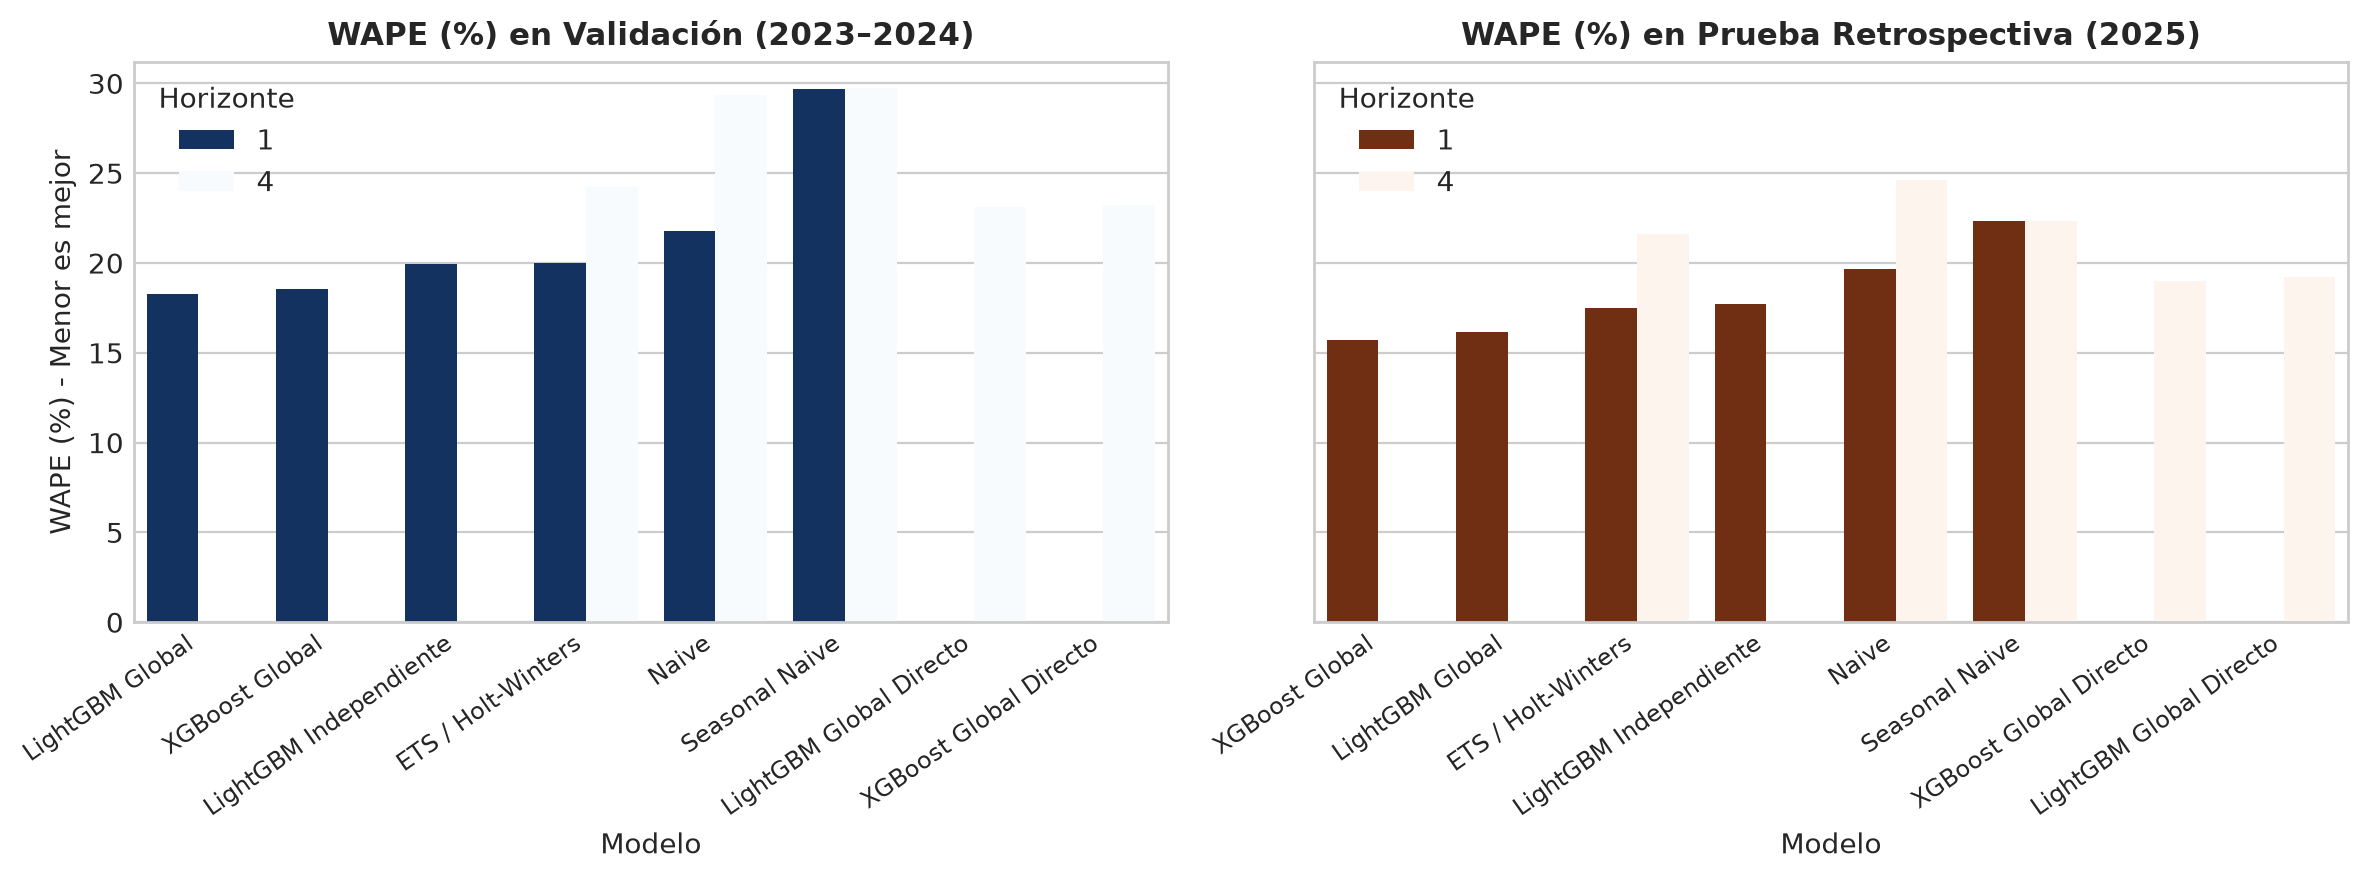
\includegraphics[width=0.94\linewidth,height=0.29\textheight,keepaspectratio]{figuras/04_comparacion_modelos_wape.png}
\caption{Error WAPE de los modelos comparados en ambos horizontes y particiones temporales.}
\label{fig:modelos}
\end{figure}

La Figura~\ref{fig:pronosticos} muestra dos ejemplos de 2025: San Román a una semana y Puno a cuatro semanas. Ambos siguen el ascenso y descenso estacional, aunque se observan discrepancias en semanas de mayor variación. Las bandas representadas corresponden a \textbf{intervalos provinciales calibrados al 95\%}; la figura no compara gráficamente las bandas originales con las calibradas.

\begin{figure}[htbp]
\centering
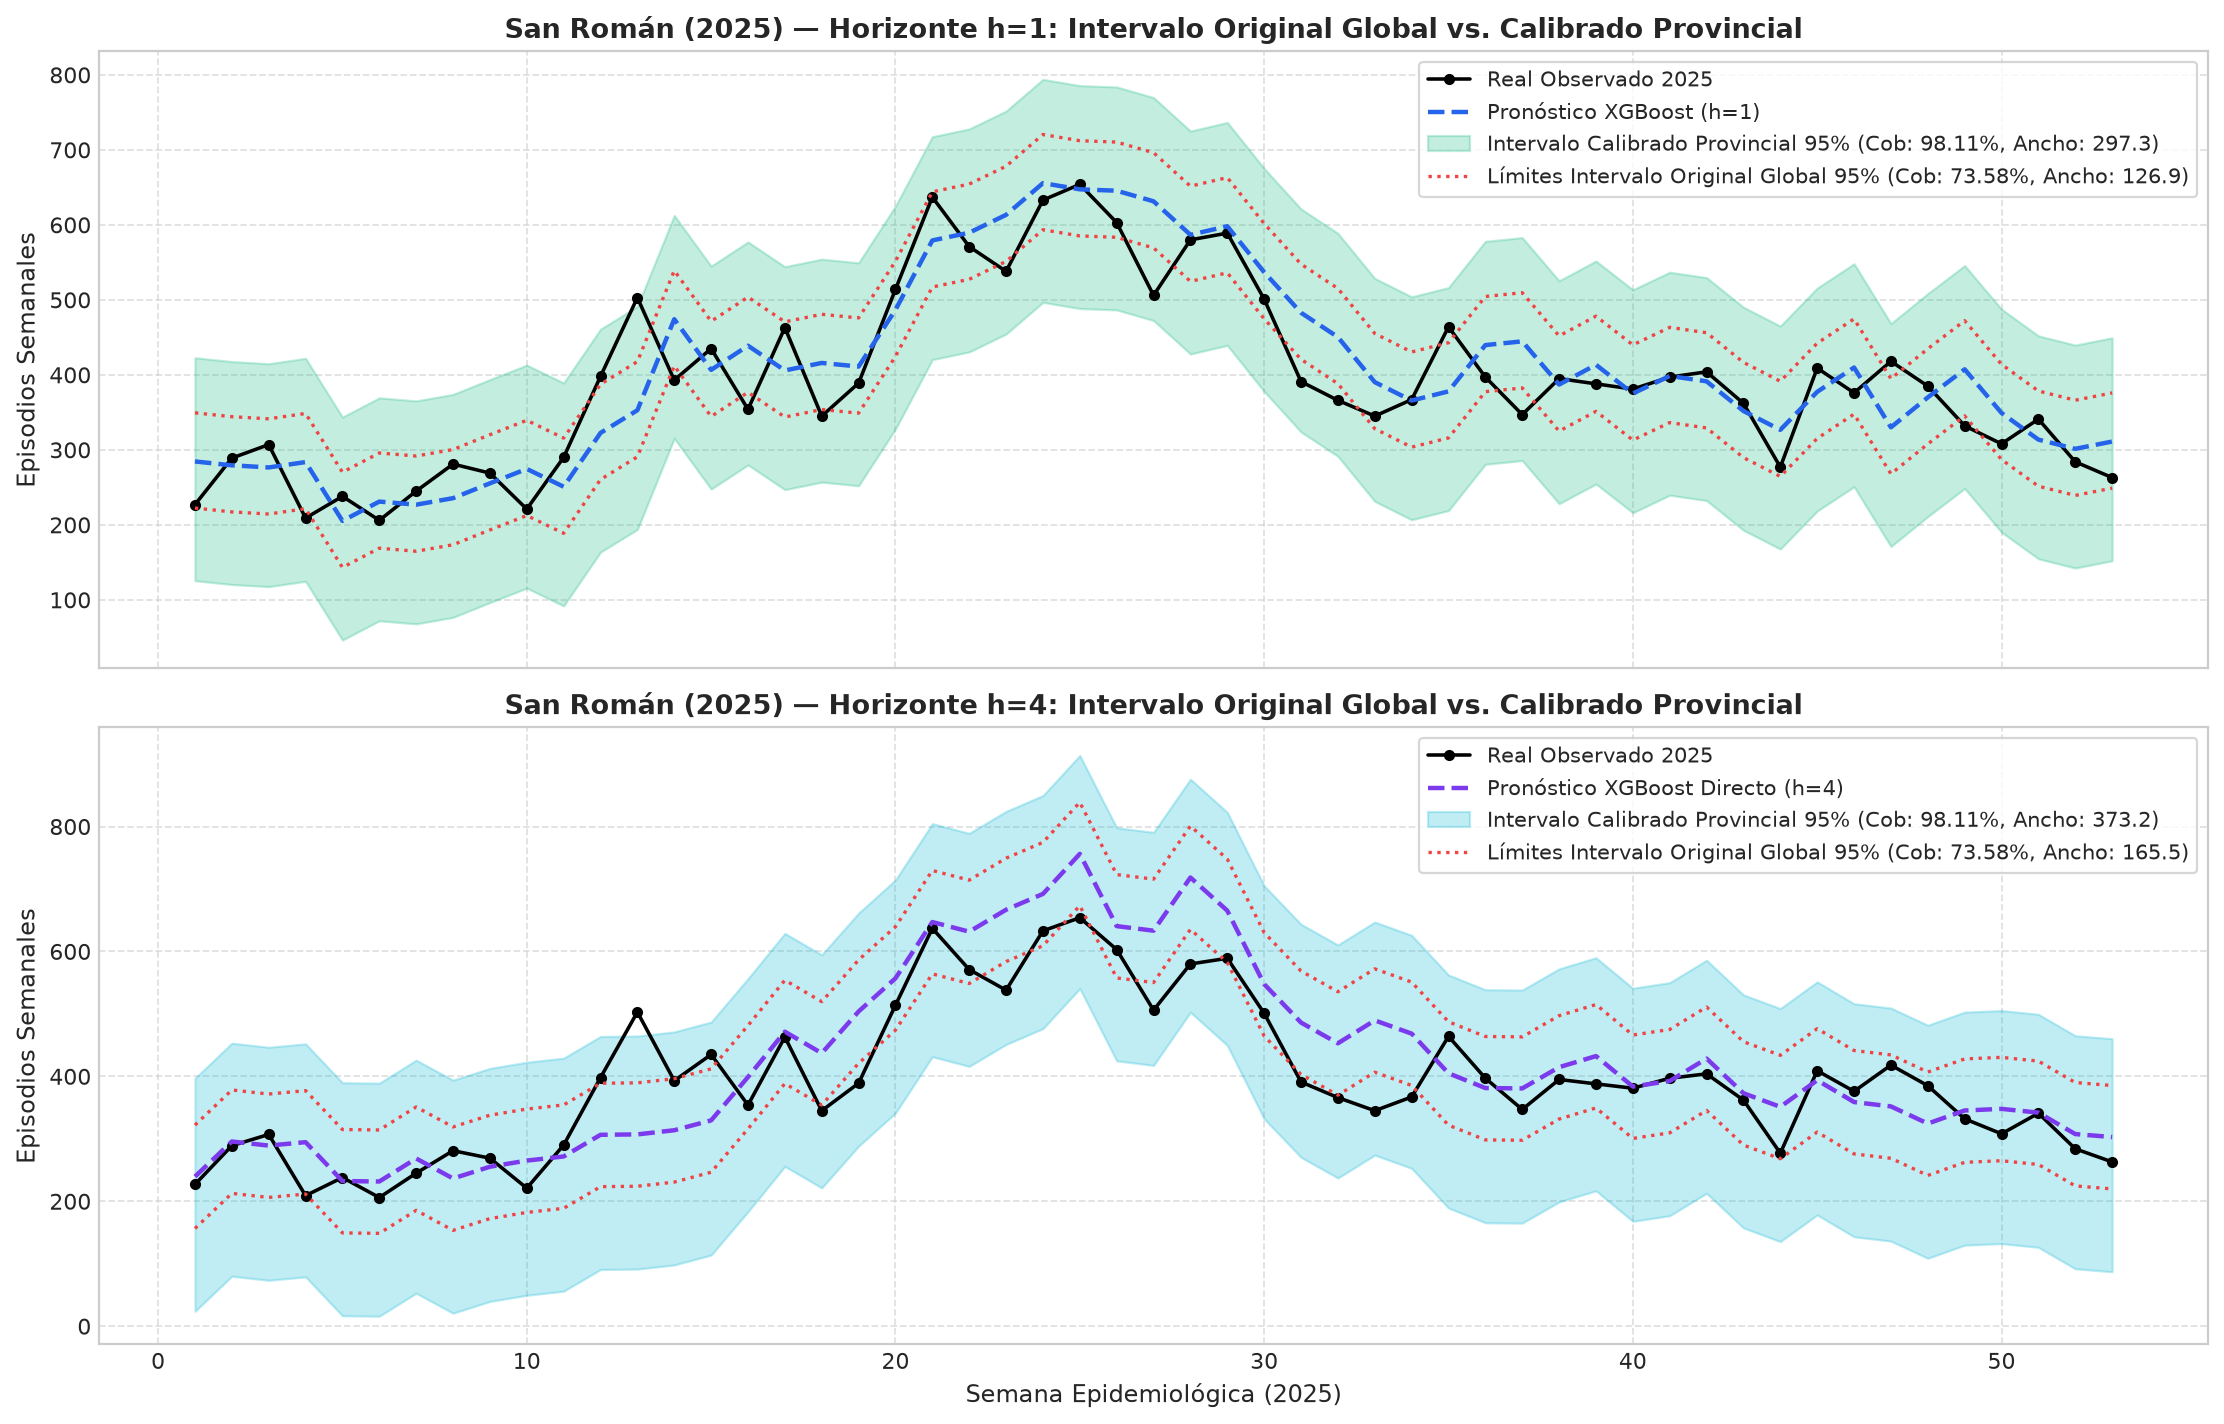
\includegraphics[width=0.95\linewidth,height=0.30\textheight,keepaspectratio]{figuras/05_series_real_vs_pronostico_2025.png}
\caption{Observaciones, pronósticos XGBoost e intervalos provinciales calibrados en 2025: San Román ($h=1$) y Puno ($h=4$).}
\label{fig:pronosticos}
\end{figure}

\subsection{Desempeño en las 13 provincias}

El WAPE departamental agrega errores de series con escalas muy distintas. La Tabla~\ref{tab:provincias} presenta los \textbf{13 resultados provinciales de XGBoost en 2025}, junto con el MAE a una semana y la cobertura de intervalos antes y después de la calibración. Todas las provincias cuentan con 53 semanas evaluadas. La Figura~\ref{fig:errorprov} permite comparar visualmente ambos horizontes.

\begin{table}[htbp]
\centering
\caption{Desempeño territorial de XGBoost en 2025: WAPE, MAE y cobertura empírica de intervalos al 95\%.}
\label{tab:provincias}
\footnotesize
\setlength{\tabcolsep}{3.6pt}
\begin{tabular}{lrrrrr}
\toprule
\textbf{Provincia} & \textbf{WAPE $h=1$} & \textbf{WAPE $h=4$} & \textbf{MAE $h=1$} & \textbf{Cob. orig.} & \textbf{Cob. calib.}\\
\midrule
San Román & 11,25 & 13,74 & 44,12 & 73,58 & 98,11\\
Puno & 11,16 & 17,45 & 27,29 & 92,45 & 96,23\\
Azángaro & 15,23 & 16,67 & 19,37 & 98,11 & 100,00\\
Melgar & 14,44 & 19,64 & 14,33 & 100,00 & 100,00\\
Carabaya & 16,46 & 16,57 & 11,93 & 100,00 & 100,00\\
Lampa & 18,98 & 21,08 & 13,81 & 100,00 & 96,23\\
Huancané & 15,79 & 21,60 & 10,18 & 100,00 & 100,00\\
Chucuito & 18,01 & 22,02 & 10,64 & 100,00 & 98,11\\
Sandia & 23,51 & 23,71 & 14,22 & 100,00 & 90,57\\
El Collao & 36,65 & 39,89 & 16,44 & 100,00 & 90,57\\
San Antonio de Putina & 33,51 & 36,35 & 10,81 & 100,00 & 100,00\\
Yunguyo & 24,49 & 23,47 & 6,58 & 100,00 & 100,00\\
Moho & 46,07 & 50,32 & 6,13 & 100,00 & 90,57\\
\midrule
\textbf{Agregado regional} & \textbf{15,72} & \textbf{18,97} & \textbf{15,84} & \textbf{97,24} & \textbf{96,95}\\
\bottomrule
\end{tabular}
\par\vspace{2pt}
\raggedright\footnotesize \emph{Nota:} Coberturas originales y calibradas corresponden a $h=1$; el agregado regional se calcula sobre las observaciones, no como promedio simple de WAPE provinciales.
\end{table}

\begin{figure}[htbp]
\centering
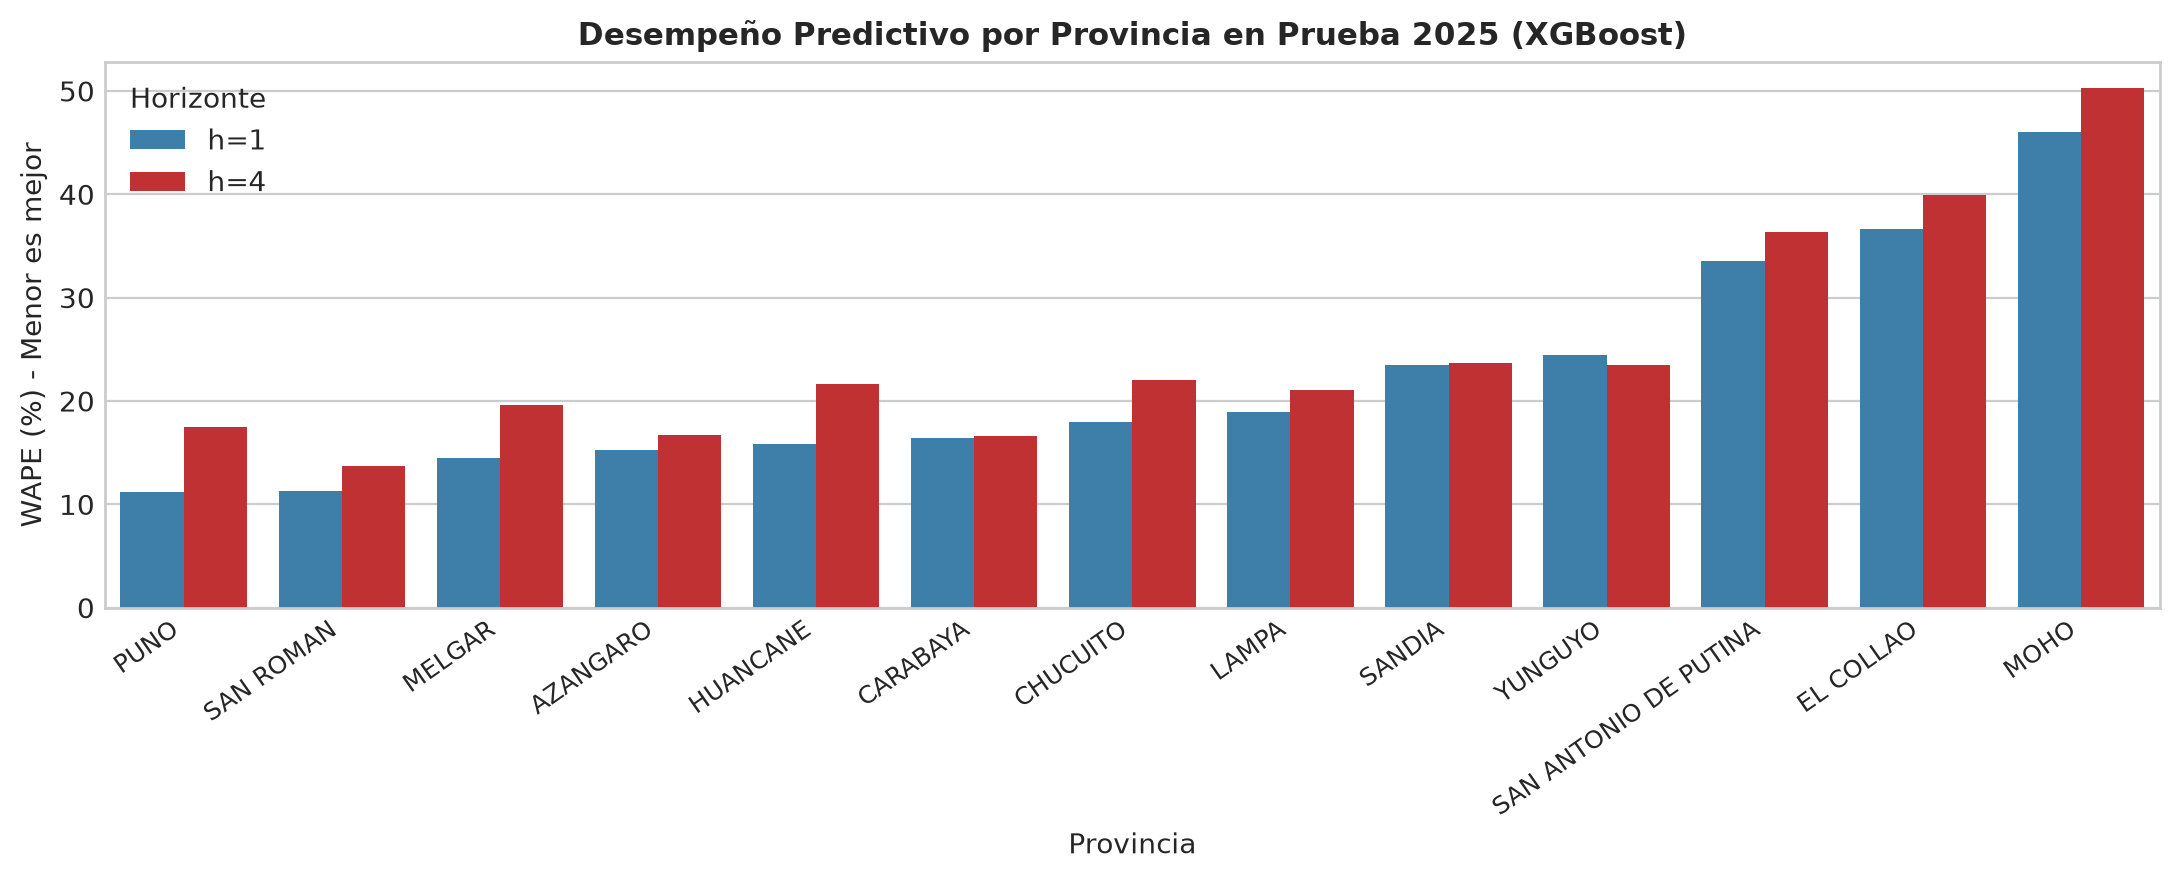
\includegraphics[width=0.95\linewidth,height=0.27\textheight,keepaspectratio]{figuras/06_desempeno_error_por_provincia.png}
\caption{WAPE provincial de XGBoost en la prueba 2025, para $h=1$ y $h=4$.}
\label{fig:errorprov}
\end{figure}

La precisión relativa es favorable en Puno y San Román (WAPE próximo al 11\% a una semana), pero el error crece en provincias de bajo volumen: \textbf{Moho alcanza 46,07\%} y \textbf{El Collao 36,65\%}. En Moho el MAE fue de solo \textbf{6,13 episodios}, de modo que el porcentaje elevado debe leerse junto con un denominador pequeño. Por el contrario, San Román presentó un MAE de 44,12 episodios aun con WAPE bajo. Estos contrastes muestran por qué el indicador agregado no sustituye al diagnóstico provincial. La relación observada entre volumen y error no permite atribuir sus diferencias a una causa poblacional o asistencial específica.

\subsection{Optimización y experimentos complementarios}

\subsubsection{Estabilidad temporal: Rolling-Origin}

Se evaluaron cinco ventanas expansivas, cada una con entrenamiento hasta el año previo y prueba en 2020--2024. El procedimiento refleja la sensibilidad del pronóstico a períodos distintos, aunque las configuraciones ya habían sido elegidas utilizando 2023--2024; por ello se interpreta como \textbf{análisis retrospectivo de estabilidad}, no como validación independiente de hiperparámetros. Los tamaños efectivos y WAPE se resumen en la Tabla~\ref{tab:rolling} y la Figura~\ref{fig:rolling}.

\begin{table}[htbp]
\centering
\caption{Validación Rolling-Origin: tamaños efectivos y WAPE (\%) por año de prueba.}
\label{tab:rolling}
\footnotesize
\setlength{\tabcolsep}{3.5pt}
\begin{tabular}{rrrrrrr}
\toprule
\textbf{Año} & \textbf{$N_{\mathrm{train}}$} & \textbf{$N_{\mathrm{test}}$} & \textbf{LGB $h=1$} & \textbf{XGB $h=1$} & \textbf{LGB $h=4$} & \textbf{XGB $h=4$}\\
\midrule
2020 & 12\,785 & 658 & 57,674 & 51,651 & 112,446 & 103,262\\
2021 & 13\,443 & 666 & 24,734 & 23,836 & 33,596 & 32,382\\
2022 & 14\,109 & 676 & 20,133 & 19,732 & 28,392 & 28,126\\
2023 & 14\,785 & 671 & 19,984 & 20,270 & 27,091 & 26,983\\
2024 & 15\,456 & 676 & 16,647 & 16,831 & 19,389 & 19,522\\
\bottomrule
\end{tabular}
\end{table}

\begin{figure}[htbp]
\centering
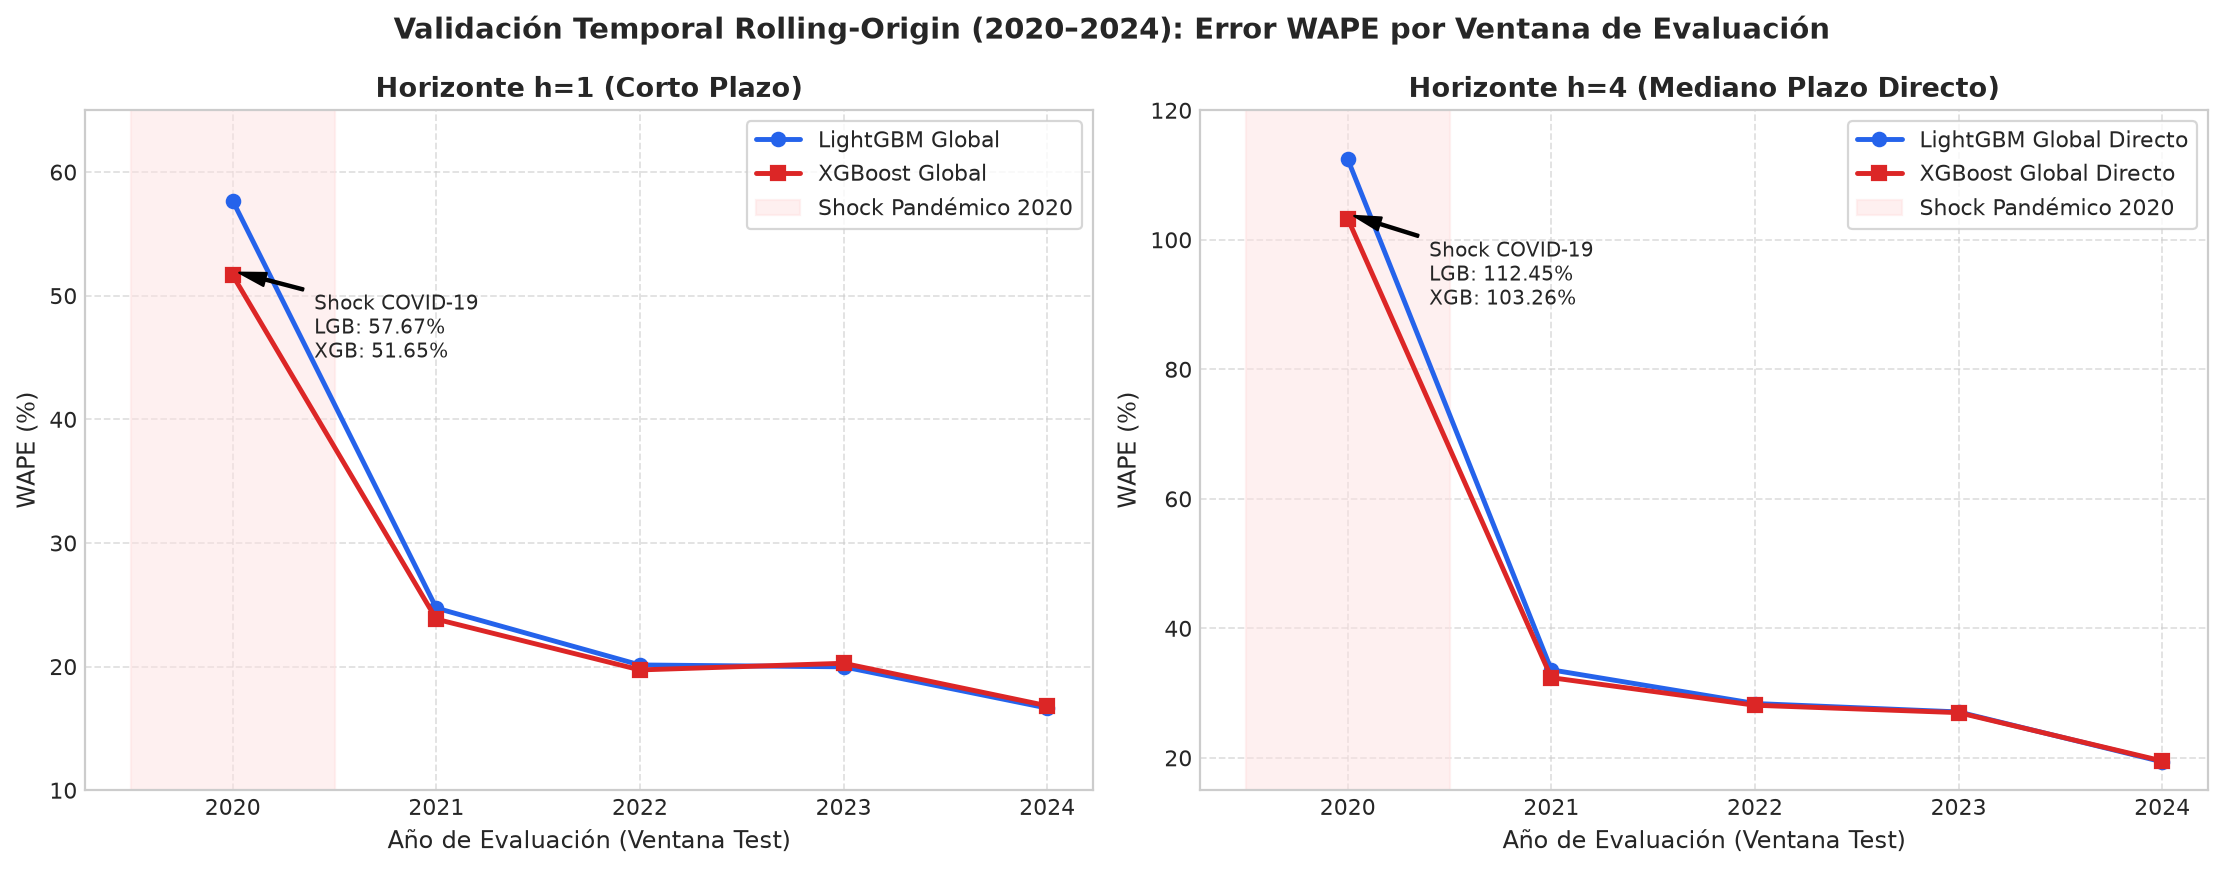
\includegraphics[width=0.94\linewidth,height=0.28\textheight,keepaspectratio]{figuras/08_validacion_rolling_origin_wape.png}
\caption{Variación del WAPE de LightGBM y XGBoost durante cinco años de prueba, en ambos horizontes.}
\label{fig:rolling}
\end{figure}

El mayor deterioro se produjo en 2020: XGBoost alcanzó WAPE de \textbf{51,651\%} ($h=1$) y \textbf{103,262\%} ($h=4$), cuando la notificación cambió de régimen. Entre 2021 y 2024 los errores disminuyeron en términos generales, sin una trayectoria estrictamente monótona. En las cinco ventanas, XGBoost obtuvo WAPE agregado de \textbf{22,480\%} en $h=1$ frente a \textbf{23,106\%} de LightGBM; los IQR interanuales, calculados con percentiles lineales, fueron 4,104 y 4,750 puntos porcentuales, respectivamente. Estas diferencias describen estabilidad observada, no garantizan desempeño futuro.

\subsubsection{Búsqueda de hiperparámetros y función de conteo}

La búsqueda original evaluó cinco configuraciones por algoritmo y horizonte. Posteriormente, Optuna TPE probó \textbf{120 ensayos} en total (30 por cada una de cuatro combinaciones), con semilla 42 y objetivo de minimizar WAPE en validación 2023--2024. Mejoró ligeramente tres combinaciones, con un máximo de \textbf{0,281 puntos porcentuales}; no existía un umbral de mejora fijado de antemano y se mantuvieron los modelos originales por sencillez y trazabilidad. En LightGBM, \texttt{subsample} no actuó porque \texttt{subsample\_freq=0}; por ello ese parámetro explorado no aportó variación efectiva.

Se comparó también la pérdida cuadrática original (L2) con los objetivos Poisson de LightGBM y XGBoost, manteniendo los otros hiperparámetros. La Tabla~\ref{tab:optimizacion} muestra que \textbf{Poisson no redujo el WAPE agregado en ninguna combinación}. En subconjuntos de temporada alta se observaron cambios favorables de sesgo, pero los errores relativos empeoraron para conteos muy reducidos. El VMR marginal no demuestra por sí mismo por qué ocurrió esta diferencia.

\begin{table}[htbp]
\centering
\caption{Comparación de WAPE (\%) en validación 2023--2024 según estrategia experimental.}
\label{tab:optimizacion}
\small
\begin{tabular}{llrrr}
\toprule
\textbf{Algoritmo} & \textbf{$h$} & \textbf{L2 original} & \textbf{Optuna} & \textbf{Poisson}\\
\midrule
LightGBM & 1 & \textbf{18,247} & 18,287 & 18,452\\
XGBoost & 1 & 18,563 & \textbf{18,412} & 18,631\\
LightGBM & 4 & 23,135 & \textbf{22,973} & 23,254\\
XGBoost & 4 & 23,236 & \textbf{22,955} & 23,341\\
\bottomrule
\end{tabular}
\end{table}

\subsubsection{Calibración provincial de intervalos}

La cobertura de los intervalos globales originales en 2025 parecía adecuada al agregarse por departamento, pero era desigual por provincia. Para explorar una alternativa, se calcularon cuantiles de los residuos fuera de muestra de \textbf{2023--2024} por provincia y horizonte: 104 observaciones por provincia, excepto Melgar (99). Los límites se mantuvieron fijos al evaluar 2025 y se truncaron en cero cuando correspondía al conteo. Estos intervalos empíricos no poseen una garantía conformal exacta bajo dependencia temporal.

\begin{table}[htbp]
\centering
\caption{Calibración de intervalos al 95\%: cobertura, amplitud media y Winkler Score en 2025.}
\label{tab:calibracion}
\footnotesize
\setlength{\tabcolsep}{4pt}
\begin{tabular}{llrrr}
\toprule
\textbf{Modelo} & \textbf{$h$} & \textbf{Cobertura: orig. $\to$ calib.} & \textbf{Ancho: orig. $\to$ calib.} & \textbf{Winkler: orig. $\to$ calib.}\\
\midrule
LightGBM & 1 & 97,24 $\to$ 96,66 & 117,03 $\to$ 99,01 & 150,51 $\to$ 112,89\\
XGBoost & 1 & 97,24 $\to$ 96,95 & 115,35 $\to$ 101,67 & 140,64 $\to$ 111,97\\
LightGBM & 4 & 96,37 $\to$ 97,82 & 138,88 $\to$ 125,32 & 174,29 $\to$ 132,82\\
XGBoost & 4 & 96,95 $\to$ 97,39 & 142,80 $\to$ 124,90 & 178,45 $\to$ 137,17\\
\bottomrule
\end{tabular}
\end{table}

La Tabla~\ref{tab:provincias} permite localizar el efecto en cada provincia para XGBoost $h=1$: en \textbf{San Román} la cobertura pasó de \textbf{73,58\% a 98,11\%}, a costa de ampliar la banda media de \textbf{126,95 a 297,31 episodios}. En \textbf{Moho} el ancho disminuyó de \textbf{79,72 a 24,33 episodios}, con cobertura de 90,57\%. En el conjunto de modelos el Winkler Score agregado descendió más del 20\%, pero hubo deterioros provinciales, como en Puno y Azángaro. La calibración es, por tanto, un \textbf{resultado experimental prometedor}, pendiente de mayor validación temporal antes de sustituir los intervalos definitivos.

\subsection{Analítica prescriptiva: escenarios de referencia}

Para mostrar una posible aplicación a decisiones de planificación se compararon pronósticos de XGBoost a una semana con \textbf{dos umbrales hipotéticos} para San Román en 2025. Con una referencia fija de \textbf{300 episodios semanales}, el pronóstico la superó durante \textbf{42 semanas consecutivas} (SE 12--53), con una diferencia máxima de \textbf{355,65 episodios} en la SE 24. Cuando la referencia fue la \textbf{media histórica de 422,6 episodios}, hubo \textbf{17 semanas no consecutivas} por encima, 13 de ellas seguidas entre las SE 20 y 32; la diferencia máxima fue \textbf{233,05 episodios}. La Figura~\ref{fig:prescripcion} muestra la serie de San Román y una comparación territorial ilustrativa.

\begin{figure}[htbp]
\centering
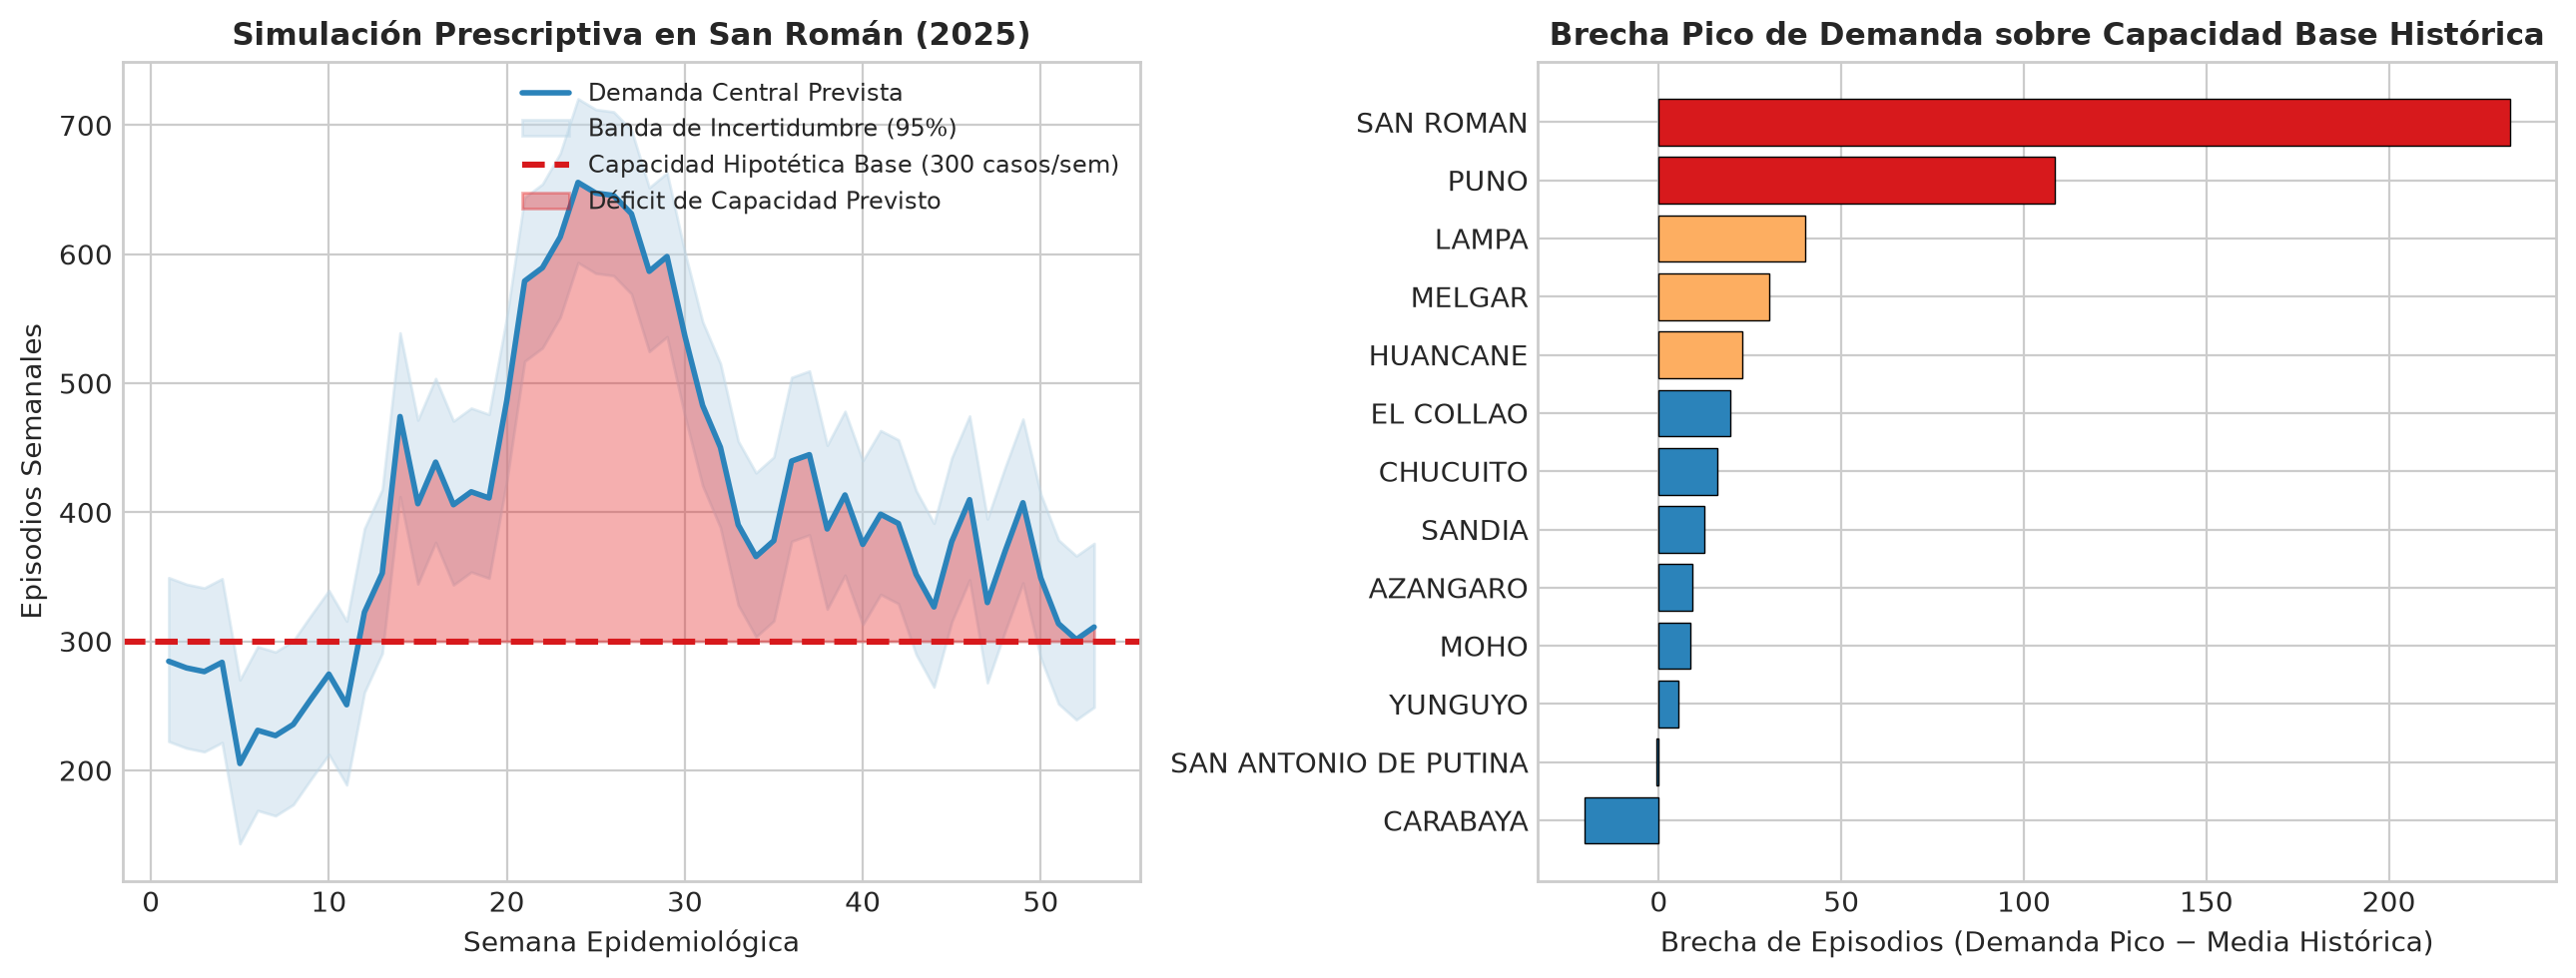
\includegraphics[width=0.95\linewidth,height=0.29\textheight,keepaspectratio]{figuras/07_simulacion_prescriptiva_capacidad.png}
\caption{Escenario de umbral fijo para San Román y brechas máximas frente a referencias históricas provinciales.}
\label{fig:prescripcion}
\end{figure}

Estas diferencias son \textbf{brechas simuladas entre episodios previstos y referencias elegidas}, no consultas no atendidas ni déficits sanitarios comprobados. El modelo no dispone de capacidad instalada, recursos humanos o inventarios reales de los establecimientos; por ello sus resultados no justifican por sí solos decisiones de contratación o compra de medicamentos.

% Discusión
\section{Discusión}

El resultado más relevante no es únicamente la mejora del WAPE frente a líneas base, sino la \textbf{heterogeneidad de desempeño}: las provincias de mayor volumen pueden presentar errores porcentuales bajos y, simultáneamente, errores absolutos importantes; las de pocos episodios pueden mostrar el patrón opuesto. El caso de San Román también revela que una cobertura global del 95\% o superior no asegura bandas de incertidumbre adecuadas en cada territorio. Para aplicaciones operativas deben examinarse en conjunto error, cobertura y amplitud.

La validación temporal muestra otra restricción: un modelo entrenado en un período histórico relativamente estable puede fallar ante cambios abruptos de notificación. Además, las configuraciones elegidas con validación 2023--2024 no convierten Rolling-Origin en un test completamente independiente. El año 2025 se reservó originalmente para prueba, pero sus resultados fueron examinados durante las fases posteriores; por ello no constituye una evaluación ciega para seleccionar nuevas calibraciones. Diferencias pequeñas entre LightGBM y XGBoost necesitan contrastes emparejados adicionales para sostener afirmaciones de superioridad estadística.

Se estudió también la viabilidad de integrar población del INEI y meteorología de NASA POWER y SENAMHI. \textbf{Ninguna de esas fuentes se incorporó a los modelos presentados}. La población menor de cinco años podría permitir tasas de episodios notificados si se consigue un denominador provincial anual fiable; la meteorología exigiría comprobar representación espacial y disponibilidad de información en cada origen de predicción. Se preservó así el registro epidemiológico como fuente única del análisis implementado.

% Conclusiones
\section{Conclusiones}

El análisis de las 13 provincias de Puno permitió consolidar un panel de 17\,641 observaciones semanales, preservando 153 ausencias de notificación, e identificar una marcada concentración territorial y estacionalidad. Los modelos globales superaron a las referencias evaluadas; XGBoost obtuvo WAPE de 15,72\% a una semana y 18,97\% a cuatro semanas en 2025, aunque su desempeño varió entre períodos y provincias. La calibración provincial mejoró el Winkler Score agregado y la cobertura en San Román, a costa de intervalos más amplios y resultados desiguales en otros territorios, por lo que requiere validación adicional. Optuna produjo mejoras marginales y Poisson no redujo el WAPE agregado. Finalmente, la simulación prescriptiva mostró cómo utilizar los pronósticos para explorar escenarios de planificación, sin representar capacidades sanitarias reales ni establecer relaciones causales.


% Referencias
\section{Referencias}
\begin{enumerate}[label={\arabic*.}]
\item Centro Nacional de Epidemiología, Prevención y Control de Enfermedades (CDC Perú/MINSA). \textit{Vigilancia epidemiológica de Infecciones Respiratorias Agudas (IRA)}. Plataforma Nacional de Datos Abiertos. \url{https://www.datosabiertos.gob.pe/dataset/vigilancia-epidemiologica-de-infecciones-respiratorias-agudas-ira}.
\item Chen, T. y Guestrin, C. (2016). \textit{XGBoost: A Scalable Tree Boosting System}. \url{https://doi.org/10.1145/2939672.2939785}.
\item Ke, G. et al. (2017). \textit{LightGBM: A Highly Efficient Gradient Boosting Decision Tree}. Advances in Neural Information Processing Systems, 30.
\item Gneiting, T. y Raftery, A. E. (2007). \textit{Strictly Proper Scoring Rules, Prediction, and Estimation}. \url{https://doi.org/10.1198/016214506000001437}.
\item Hyndman, R. J. y Athanasopoulos, G. (2021). \textit{Forecasting: Principles and Practice}, tercera edición. \url{https://otexts.com/fpp3/}.
\item Instituto Nacional de Estadística e Informática (INEI). \textit{Perú: Estimaciones y proyecciones de población departamental, por años calendario y edad simple, 1995--2030}. Boletín Especial N.\textsuperscript{o} 25.
\item NASA. \textit{Prediction of Worldwide Energy Resources (POWER)}. \url{https://power.larc.nasa.gov/}.
\item Servicio Nacional de Meteorología e Hidrología del Perú (SENAMHI). \textit{Portal institucional}. \url{https://www.gob.pe/senamhi}.
\end{enumerate}

\end{document}
